\chapter{Output from Dakota}\label{output}

\section{Overview of Output Formats}\label{output:overview}

While Dakota primarily targets complex numerical simulation codes run
on massively parallel supercomputers, Dakota's output focuses on
succinct, text-based reporting of the iterations and function
evaluations performed by an algorithm. In a number of contexts, Dakota
generates tabular output useful for data analysis and visualization
with external tools.  Unix versions of Dakota have an optional basic
graphical output capability that can be useful as a monitoring tool.
The Dakota GUI increasingly provides replacement visualization
facilities.

\section{Standard Output}\label{output:standard}

Dakota prints information on algorithm progress, function evaluations,
and summary results to standard out and error (screen, terminal, or
console) as it runs.  Detailed information for a function evaluation
may include an evaluation number, parameter values, execution syntax,
the active set vector, and the response data set.  This output may be
redirected to a file using the command-line options described in
Section~\ref{tutorial:installation:running}.

Here, optimization of the ``container'' problem (see
Chapter~\ref{additional}) is used as an example to describe Dakota
output. The input file shown in Figure~\ref{output:incont} specifies
one equality constraint, and that Dakota's finite difference algorithm
will provide central difference numerical gradients to the NPSOL
optimizer.
\begin{figure}
  \begin{small}
    \begin{bigbox}
      \verbatimtabinput[8]{container_opt_npsol.in}
    \end{bigbox}
  \end{small}
  \caption{Dakota input file for the ``container'' test problem --
see \protect\path{dakota/share/dakota/examples/users/container_opt_npsol.in} }
  \label{output:incont}
\end{figure}

\clearpage

A partial listing of the Dakota output for the container optimization
example follows:
\begin{small}
\begin{verbatim}
Dakota version 5.4+ (stable) released May  2 2014.
Subversion revision 2508 built May  2 2014 15:26:14.
Running MPI Dakota executable in serial mode.
Start time: Fri May  2 15:38:11 2014

----------------------------------------------------------------
Begin DAKOTA input file
/home/user/dakota/build/examples/users/container_opt_npsol.in
----------------------------------------------------------------
# Dakota Input File: container_opt_npsol.in
environment

<SNIP>

---------------------
End DAKOTA input file
---------------------

Using Dakota input file '/home/user/dakota/build/examples/users/container_opt_npsol.in'
Writing new restart file dakota.rst

>>>>> Executing environment.

>>>>> Running npsol_sqp iterator.

------------------------------------------
Begin Dakota derivative estimation routine
------------------------------------------

>>>>> Initial map for analytic portion of response:

---------------------
Begin Evaluation    1
---------------------
Parameters for evaluation 1:
                      4.5000000000e+00 H
                      4.5000000000e+00 D

blocking fork: container container.in.1 container.out.1

Active response data for evaluation 1:
Active set vector = { 1 1 }
                      1.0713145108e+02 obj_fn
                      8.0444076396e+00 nln_eq_con_1


>>>>> Dakota finite difference gradient evaluation for x[1] + h:

---------------------
Begin Evaluation    2
---------------------
Parameters for evaluation 2:
                      4.5045000000e+00 H
                      4.5000000000e+00 D

blocking fork: container container.in.2 container.out.2

Active response data for evaluation 2:
Active set vector = { 1 1 }
                      1.0719761302e+02 obj_fn
                      8.1159770472e+00 nln_eq_con_1


>>>>> Dakota finite difference gradient evaluation for x[1] - h:

---------------------
Begin Evaluation    3
---------------------
Parameters for evaluation 3:
                      4.4955000000e+00 H
                      4.5000000000e+00 D

blocking fork: container container.in.3 container.out.3

Active response data for evaluation 3:
Active set vector = { 1 1 }
                      1.0706528914e+02 obj_fn
                      7.9728382320e+00 nln_eq_con_1


>>>>> Dakota finite difference gradient evaluation for x[2] + h:

---------------------
Begin Evaluation    4
---------------------
Parameters for evaluation 4:
                      4.5000000000e+00 H
                      4.5045000000e+00 D

blocking fork: container container.in.4 container.out.4

Active response data for evaluation 4:
Active set vector = { 1 1 }
                      1.0727959301e+02 obj_fn
                      8.1876180243e+00 nln_eq_con_1


>>>>> Dakota finite difference gradient evaluation for x[2] - h:

---------------------
Begin Evaluation    5
---------------------
Parameters for evaluation 5:
                      4.5000000000e+00 H
                      4.4955000000e+00 D

blocking fork: container container.in.5 container.out.5

Active response data for evaluation 5:
Active set vector = { 1 1 }
                      1.0698339109e+02 obj_fn
                      7.9013403937e+00 nln_eq_con_1


>>>>> Total response returned to iterator:

Active set vector = { 3 3 } Deriv vars vector = { 1 2 }
                      1.0713145108e+02 obj_fn
                      8.0444076396e+00 nln_eq_con_1
 [  1.4702653619e+01  3.2911324639e+01 ] obj_fn gradient
 [  1.5904312809e+01  3.1808625618e+01 ] nln_eq_con_1 gradient


<SNIP>


>>>>> Dakota finite difference gradient evaluation for x[2] - h:

---------------------
Begin Evaluation   40
---------------------
Parameters for evaluation 40:
                      4.9873894231e+00 H
                      4.0230575428e+00 D

blocking fork: container container.in.40 container.out.40

Active response data for evaluation 40:
Active set vector = { 1 1 }
                      9.8301287596e+01 obj_fn
                     -1.2698647501e-01 nln_eq_con_1


>>>>> Total response returned to iterator:

Active set vector = { 3 3 } Deriv vars vector = { 1 2 }
                      9.8432498116e+01 obj_fn
                     -9.6918029158e-12 nln_eq_con_1
 [  1.3157517860e+01  3.2590159623e+01 ] obj_fn gradient
 [  1.2737124497e+01  3.1548877601e+01 ] nln_eq_con_1 gradient



NPSOL exits with INFORM code = 0 (see "Interpretation of output" section in NPSOL manual)

NOTE: see Fortran device 9 file (fort.9 or ftn09)
      for complete NPSOL iteration history.
<<<<< Function evaluation summary: 40 total (40 new, 0 duplicate)
<<<<< Best parameters          =
                      4.9873894231e+00 H
                      4.0270846274e+00 D
<<<<< Best objective function  =
                      9.8432498116e+01
<<<<< Best constraint values   =
                     -9.6918029158e-12
<<<<< Best data captured at function evaluation 36


<<<<< Iterator npsol_sqp completed.
<<<<< Environment execution completed.
DAKOTA execution time in seconds:
  Total CPU        =       0.03 [parent =   0.023997, child =   0.006003]
  Total wall clock =   0.090703
\end{verbatim}
\end{small}

The output begins with information on the Dakota version, compilation
date, and run mode.  It then echos the user input file before
proceeding to execution phase.  The lines following ``\texttt{>>>>>
  Running npsol\_sqp iterator.}''  show Dakota performing function
evaluations 1--5 that have been requested by NPSOL. Evaluations 6
through 39 have been omitted from the listing for brevity.

Immediately following the line ``\texttt{Begin Function Evaluation
  1}'', the initial values of the design variables, the syntax of the
blocking fork function evaluation, and the resulting objective and
constraint function values returned by the simulation are listed.  The
values of the design variables are labeled with the tags \texttt{H}
and \texttt{D}, respectively, according to the descriptors given in
the input file, Figure~\ref{output:incont}.  The values of the
objective function and volume constraint are labeled with the tags
\texttt{obj\_fn} and \texttt{nln\_eq\_con\_1}, respectively. Note that
the initial design parameters are infeasible since the equality
constraint is violated ($\ne 0$). However, by the end of the run, the
optimizer finds a design that is both feasible and optimal for this
example. Between the design variables and response values, the content
of the system call to the simulator is displayed as
``\texttt{(container container.in.1 container.out.1)}'', with
\path{container} being the name of the simulator and
\path{container.in.1} and \path{container.out.1} being the names
of the parameters and results files, respectively.

Just preceding the output of the objective and constraint function
values is the line ``\texttt{Active set vector = \{1 1\}}''. The
active set vector indicates the types of data that are required from
the simulator for the objective and constraint functions, and values
of ``\texttt{1}'' indicate that the simulator must return values for
these functions (gradient and Hessian data are not required). For more
information on the active set vector, see Section~\ref{variables:asv}.

Since finite difference gradients have been specified, Dakota computes
their values by making additional function evaluation requests to the
simulator at perturbed parameter values. Examples of the
gradient-related function evaluations have been included in the sample
output, beginning with the line that reads ``\texttt{>>>>> Dakota
  finite difference evaluation for x[1] + h:}''. The resulting finite
difference gradients are listed after function evaluation 5 beginning
with the line ``\texttt{>>>>> Total response returned to iterator:}''.
Here, another active set vector is displayed in the Dakota output
file. The line ``\texttt{Active set vector = \{ 3 3 \}}'' indicates
that the total response resulting from the finite differencing
contains function values and gradients.

The final lines of the Dakota output, beginning with the line
``\texttt{<<<<< Function evaluation summary:}'', summarize the
results of the optimization study. The best values of the optimization
parameters, objective function, and volume constraint are presented
along with the function evaluation number where they occurred, total
function evaluation counts, and a timing summary. In the end, the
objective function has been minimized and the equality constraint has
been satisfied (driven to zero within the constraint tolerance).

The Dakota results may be intermixed with iteration information from
the NPSOL library. For example lines with the heading ``\texttt{Majr
  Minr Step Fun Merit function Norm gZ Violtn nZ Penalty Conv}'' come
from Fortran write statements within NPSOL. The output is mixed since
both Dakota and NPSOL are writing to the same standard output
stream. The relative locations of these output contributions can vary
depending on the specifics of output buffering and flushing on a
particular platform and depending on whether or not the standard
output is being redirected to a file. In some cases, output from the
optimization library may appear on each iteration (as in this
example), and in other cases, it may appear at the end of the Dakota
output. Finally, a more detailed summary of the NPSOL iterations is
written to the Fortran device 9 file (e.g., \texttt{fort.9} or
\texttt{ftn09}).

\section{Tabular Output Data}\label{output:tabular}

In a number of contexts, Dakota can output information in a
whitespace-separated columnar data file, a tabular data file.  The
most common usage, to capture the iteration history in a tabular file,
is enabled by including the keyword \texttt{tabular\_data} in the
\texttt{environment} specification (see
Figure~\ref{output:incont}). This output format facilitates the
transfer of Dakota's iteration history data to external mathematical
analysis and/or graphics plotting packages (e.g., MATLAB, TECplot,
Excel, S-plus, Minitab).

The default file name for the top-level tabular output data is
``\path{dakota_tabular.dat},'' though \texttt{tabular\_data\_file}
allows specification of an alternate name.  Example tabular output
from the ``container'' optimization problem is shown in
Figure~\ref{output:tabcont}. This annotated tabular format (see
Section~\ref{input:tabularformat}) file contains the complete history
of data requests from NPSOL (8 requests map into a total of 40
function evaluations when including the central finite
differencing). The first column is the data request number, the second
column is the interface ID (which is \texttt{NO\_ID} if the user does
not specify a name for the interface), the third and fourth columns
are the design parameter values (labeled in the example as
``\texttt{H}'' and ``\texttt{D}''), the fifth column is the objective
function (labeled ``\texttt{obj\_fn}''), and the sixth column is the
nonlinear equality constraint (labeled ``\texttt{nln\_eq\_con\_1}'').

\begin{figure}
\begin{bigbox}
\begin{small}
\begin{verbatim}
%eval_id interface             H              D         obj_fn   nln_eq_con_1 
       1     NO_ID           4.5            4.5    107.1314511     8.04440764 
       2     NO_ID   5.801246882    3.596476363    94.33737399    -4.59103645 
       3     NO_ID   5.197920019    3.923577479     97.7797214  -0.6780884711 
       4     NO_ID   4.932877133    4.044776216    98.28930566  -0.1410680284 
       5     NO_ID   4.989328733    4.026133158     98.4270019 -0.005324671422 
       6     NO_ID   4.987494493    4.027041977    98.43249058 -7.307058453e-06 
       7     NO_ID   4.987391669     4.02708372    98.43249809 -2.032538049e-08 
       8     NO_ID   4.987389423    4.027084627    98.43249812 -9.691802916e-12 
\end{verbatim}
\end{small}
\end{bigbox}
\caption{Dakota's tabular output file showing the iteration history of
the ``container'' optimization problem.} \label{output:tabcont}
\end{figure}

{\bf Attention:} The second column labeled ``\texttt{interface}'' is
new as of Dakota 6.1.  It identifies which interface was used to map
the variables to responses on each line of the tabular file (recall
that the interface defines which simulation is being run though the
\texttt{analysis\_driver} specification).  Disambiguating the
interface is important when using hybrid methods, multi-fidelity
methods, or nested models.  In more common, simpler analyses, users
typically ignore the first two columns and only focus on the columns
of inputs (variables) and outputs (responses).  \emph{To generate tabular
output in Dakota 6.0 format, use the custom-annotated format described
in Section~\ref{input:tabularformat}.}

{\bf Attention:} As of Dakota 6.1, the tabular file will include
columns for all of the variables (both active and inactive) present in
a given interface.  Previously, Dakota only wrote the ``active''
variables.  Recall that some variables may be inactive if they are not
operated on by a particular method (e.g. uncertain variables might not
be active in an optimization, design variables may not be active in a
sampling study).  The order of the variables printed out will be in
Dakota's standard variable ordering, which is indicated by the input
specification order, and summarized in the Dakota Reference Manual.

Any evaluations from Dakota's internal finite differencing are
suppressed, to facilitate rapid plotting of the most critical data.
This suppression of lower level data is consistent with the data that
is sent to the graphics windows, as described in
Section~\ref{output:graphics}. If this data suppression is
undesirable, Section~\ref{restart:utility:tabular} describes an
approach where every function evaluation, even the ones from finite
differencing, can be saved to a file in tabular format by using the
Dakota restart utility.


\section{Graphics Output}\label{output:graphics}

This section describes Dakota's legacy Unix / X Windows-based graphics
capabilities, which can help monitor study progress. Dakota plotting
and visualization capabilities are increasingly available in the
Dakota graphical user interface (GUI); see the Dakota GUI User Manual
in the documentation section of the Dakota website for additional
details.

The X Windows graphics option is invoked by including the
\texttt{graphics} flag in the environment specification of the input
file (see Figure~\ref{output:incont}). The graphics display the values
of each response function (e.g., objective and constraint functions)
and each parameter for the function evaluations in the study. As with
the tabular output described in Section~\ref{output:tabular}, internal
finite difference evaluations are suppressed in order to omit this
clutter from the graphics.  Figure~\ref{output:2dcont} shows the
optimization iteration history for the container example.

If Dakota is executed on a remote machine, the DISPLAY variable in the
user's UNIX environment~\cite{Gil92} may need to be set to the local
machine in order to display the graphics window. 

\begin{figure}
\centering
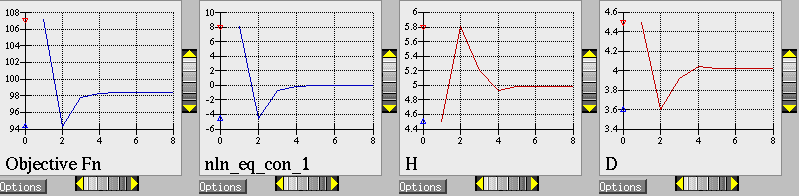
\includegraphics[width=\textwidth]{images/container_graphic}
\caption{Dakota 2D graphics for ``container'' problem showing history of
an objective function, an equality constraint, and two variables.}
\label{output:2dcont}
\end{figure}

The scroll bars which are located on each graph below and to the right
of each plot may be operated by dragging on the bars or pressing the
arrows, both of which result in expansion/contraction of the axis
scale. Clicking on the ``Options'' button results in the window shown
in Figure~\ref{output:2dcontoptions}, which allows the user to include
min/max markers on the vertical axis, vertical and horizontal axis
labels, and a plot legend within the corresponding graphics plot.  In
addition, the values of either or both axes may be plotted using a
logarithmic scale (so long as all plot values are greater than zero)
and an encapsulated postscript (EPS) file, named 
\texttt{dakota\_graphic\_\emph{i}.eps} where \emph{i} is the plot 
window number, can be created using the ``Print'' button.
\begin{figure}
\centering
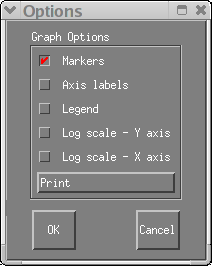
\includegraphics[scale=0.6]{images/container_graphic_options}
\caption{Options for Dakota 2D graphics.}
\label{output:2dcontoptions}
\end{figure}


\section{Error Messages Output}\label{output:error}

A variety of error messages are printed by Dakota in the event that an
error is detected in the input specification. Some of the more common
input errors, and the associated error messages, are described below.
See also the Common Specification Mistakes section in the Dakota
Reference Manual~\cite{RefMan}.

Incorrectly spelled specifications, such as 
\texttt{``numericl\_gradients''}, will result in error messages of the form:
\begin{small}
\begin{verbatim}
Input line 31: unrecognized identifier 'numericl_gradients'.
Input line 31: unrecognized identifier 'method_source'.
Input line 31: unrecognized identifier 'dakota'.
Input line 31: unrecognized identifier 'interval_type'.
Input line 31: unrecognized identifier 'central'.
Input line 31: unrecognized identifier 'fd_gradient_step_size'.
Input line 31: One of the following 4 entities
must be specified for responses...
	analytic_gradients
	mixed_gradients
	no_gradients
	numerical_gradients
\end{verbatim}
\end{small}
In this example the line numbers given are approximate, as all input
following an errant keywords is considered a single line through the
end of the block.

The input parser catches syntax errors, but not logic errors. The fact
that certain input combinations are erroneous must be detected after
parsing, at object construction time. For example, if a
\texttt{no\_gradients} specification for a response data set is
combined with selection of a gradient-based optimization method, then
this error must be detected during set-up of the optimizer (see last
line of listing):
\begin{small}
\begin{verbatim}
Error: gradient-based minimizers require a gradient specification.
\end{verbatim}
\end{small}
Many such errors can be detected earlier by running \texttt{dakota
  -check}.

Another common mistake involves a mismatch between the amount of data
expected on a function evaluation and the data returned by the user's
simulation code or driver. The available response data is specified in
the responses keyword block, and the subset of this data needed for a
particular evaluation is managed by the active set vector. For
example, if Dakota expects function values and gradients to be
returned (as indicated by an active set vector containing 3's), but
the user's simulation code only returns function values, then the
following error message is generated:
\begin{small}
\begin{verbatim}
    At EOF: insufficient data for functionGradient 1
\end{verbatim}
\end{small}

Unfortunately, descriptive error messages are not available for all
possible failure modes of Dakota. If you encounter core dumps,
segmentation faults, or other failures, please request help using the
support mechanisms described on the
\href{http://dakota.sandia.gov/}{Dakota website}.


\section{Stochastic expansion exports}\label{sec:output:pce}

Polynomial chaos expansion (PCE) methods compute coefficients for
response expansions which employ a basis of multivariate orthogonal
polynomials.  The \texttt{polynomial\_chaos} method calculates these
coefficients based on a number of approaches described in
Section~\ref{uq:expansion}).  One may output the PCE coefficients to a
file using the keyword \texttt{export\_expansion\_file =
  \emph{STRING}}.  Each row of the exported file will contain a
coefficient, followed by the multi-index indicating which basis terms
correspond to it.  Only free-form format
(Section~\ref{input:tabularformat}) is supported for this file.

When using numerical integration schemes with structured rules, Dakota
can also output the integration points and corresponding weights to a
tabular file.  This output is generated when \texttt{method output} is
\texttt{verbose} or higher.  Weights and points are printed to a file
\path{dakota_quadrature_tabular.dat} (tensor product quadrature),
\path{dakota_sparse_tabular.dat} (sparse grids), or
\path{dakota_cubature_tabular.dat} (cubature methods), with one
line per integration point.

\section{Surrogate Model Exports}

Most Dakota surrogate models, including all those implemented in
Surfpack and some stochastic expansion approaches support the keyword
\texttt{export\_approx\_points\_file = \emph{STRING}}.  When specified, any
approximate evaluations performed on the surrogate model will be
output to the specified data file.  The data file can be exported in
any of the tabular formats described in
Section~\ref{input:tabularformat} (default annotated).  This
facilitates plotting or external diagnostics of the surrogate model.

In addition, the Surfpack family of global surrogate models supports
export to a human-readable and self-documenting algebraic form, suitable for 
reuse in user-developed tools, and to non-human readable model files, 
which are intended for use with the {\tt surfpack} executable or library API. 
The \texttt{export\_model} keyword group is used to specify model export filenames 
and formats. It is fully described in the Dakota Reference Manual~\cite{RefMan}.

\section{Variables Output from Pre-run}

The pre-run mode (supported only for select methods) permits
specification of an output file to which Dakota will write parameter
(variables) data in any supported tabular format (default annotated; see
Section~\ref{input:tabularformat}) with data columns corresponding to
each variable.  This file can be generated with sampling, parameter
study, and DACE methods by invoking
\begin{small}
\begin{verbatim}
    dakota -i dakota.in -pre_run ::variables.dat
\end{verbatim}
\end{small}
for example, to output the variables (samples) in an LHS study.  If a
user adds the corresponding response values to this file, it may then
be imported using Dakota's post-run mode.  Command line pre-run will
always export in annotated format.  To export pre-run data in other
formats, specify \texttt{pre\_run} in the input file instead of at the
command-line, and provide a format option.

% LocalWords:  NPSOL npsol sqp fn nln eq infeasible differencing Majr Minr gZ
% LocalWords:  Violtn nZ Conv Fortran Fortran ftn09 MATLAB TECplot Minitab dat
% LocalWords:  dakota 2D EPS eps numericl combinations PCE multi Pre pre LHS 2D
% LocalWords:  Fortran Fortran whitespace Disambiguating analyses Surfpack sps
% LocalWords:  bsps surfpack API
